% (C) 2016 Jean Nassar. Some Rights Reserved
% Except where otherwise noted, this work is licensed under the Creative Commons Attribution-ShareAlike License, version 4
% Introduction
\chapter{Introduction}
\label{ch:intro}
%\epigraphhead{\epigraph{
  %Research is what I'm doing when I don't know what I'm doing.
%}{\textsc{Wernher von Braun}}}

This report is divided into six parts.
In \Pref{pt:overview}, the field is introduced and the purpose of the research is stated.
The background of the problem and previous research are also presented.
In \Pref{pt:implementation}, the proposal is shown and the new method's implementation is explained in detail.
In \Pref{pt:experiments}, the experiments are described, and the results and conclusions are discussed in \Pref{pt:results}.
Appendices and backmatter are in \Pref{pt:appendices} and \Pref{pt:backmatter} respectively.

\section{Unmanned Aerial Vehicles}
\subsection{History}
\Glspl{uav}, also known as drones if they have \gls{ai}, have been used since at least the mid-19th century, when the Austrian military bombarded the Italian city of Venice.\cite{monash2003}
Later developments included aerial torpedoes, assualt drones, and target drones, controlled both autonomously or remotely.
Reconnaissance drones were developed in the 1960s, and used heavily in Vietnam.
The importance of battlefield \glspl{uav} was realized in 1982 with their successful utilization by the Israeli Air Force against the Syrian Air Force over Lebanon.\cite{draganfly2009}

Modern drones have both military and civilian uses.
Multirotor \glspl{uav} have recently become common with the public, and are now used recreationally and professionally.
Some of the applications of \glspl{uav} include:

\begin{itemize}
  \item capturing photos and videos
  \item racing
  \item site inspection
  \item agriculture and land assessment
  \item news gathering
  \item police surveillance
  \item exploration
  \item search and rescue, and disaster relief
\end{itemize}

\subsection{Issues with modern drones}
A modern \gls{uav}'s payload typically consists of at least one camera, an \gls{imu} with at least six \glspl{dof}, and an autopilot to aid with stability.
More sophisiticated \glspl{uav} might have additional cameras, or sensors for altitude and distance, including sensors for \gls{3d} reconstruction of the environment.
However, these features tend to require a larger, heavier \gls{uav}, which might cost more and be less maneuverable.

Teleoperated \glspl{uav} usually use either line of sight, where the pilot has to be able to see the drone directly, or \gls{fpv}, where the pilot uses a video downlink from the drone to control it.
The downlink can be displayed in video goggles or on a standard display.
Some setups allow the camera on the drone to gimbal, while others have a zoomed-in fisheye lens, either of which can provide an immersive experience when combined with head tracking.

\begin{figure}[h]
  \centering
  \begin{subfigure}[b]{0.3\textwidth}
    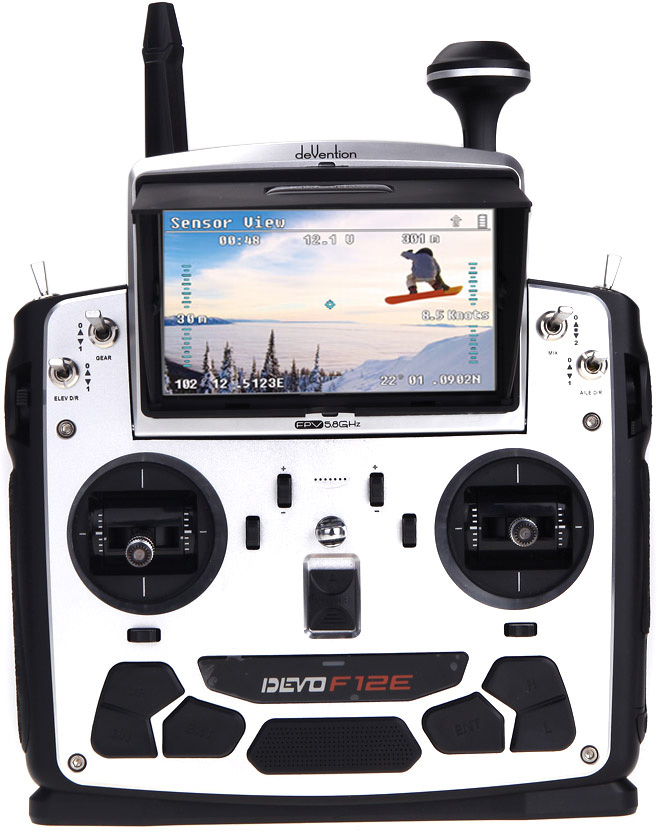
\includegraphics[width=\textwidth]{fpv_controller}
    \caption{A transmitter.\cite{fpv_controller}}
    \label{fig:fpv_controller}
  \end{subfigure}
  \hfill
  \begin{subfigure}[b]{0.3\textwidth}
    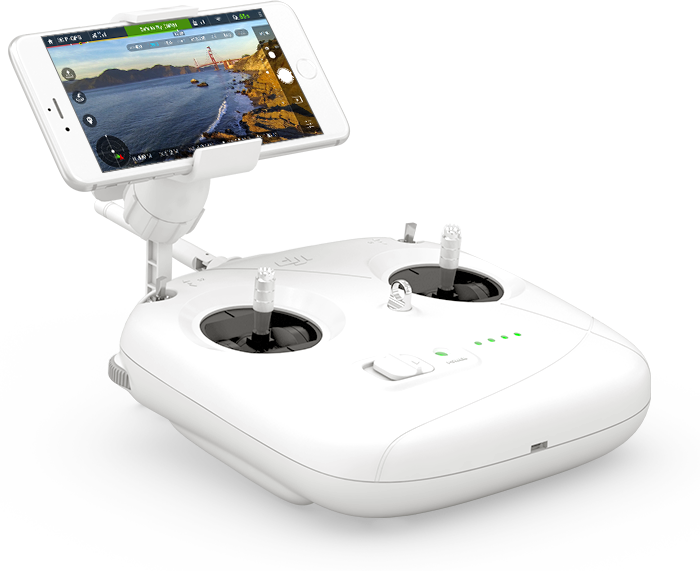
\includegraphics[width=\textwidth]{fpv_phone}
    \caption{A phone.\cite{fpv_phone}}
    \label{fig:fpv_phone}
  \end{subfigure}
  \hfill
  \begin{subfigure}[b]{0.3\textwidth}
    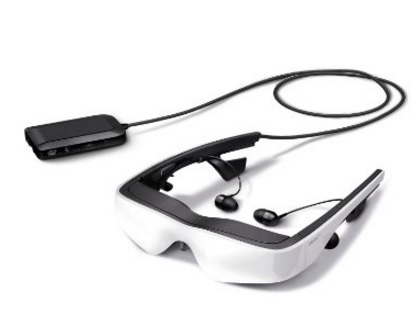
\includegraphics[width=\textwidth]{fpv_goggles}
    \caption{\gls{fpv} goggles.\cite{fpv_goggles}}
    \label{fig:fpv_goggles}
  \end{subfigure}
  \caption[\acrshort{fpv} display methods]{Various methods of displaying a \gls{fpv} feed.}
  \label{fig:fpv_various}
\end{figure}

\begin{wrapfigure}{r}{0.5\textwidth}
  \centering
  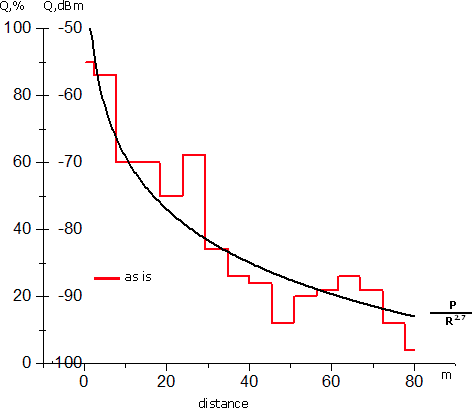
\includegraphics[width=0.48\textwidth]{ardrone_dos}
  \caption[AR.Drone signal profile]{Signal strength of the \gls{ardrone} with respect to distance. Extracted from \cite{ardrone_dos}.}
  \label{fig:ardrone_dos}
\end{wrapfigure}

\gls{fpv}, however, is normally \gls{2d}, and does not afford the user any depth perception.
As a result, loss of situational (i.e.\ spatial) awareness can occur, and the boundaries of the vehicle with respect to the environment might not be known.
This is known to have contributed to multiple crashes into the environment in the past, with powerlines damaged,\cite{latimes2015} and people gravely injured.\cite{seattletimes2015,bbcnews2015}
Incidents of \glspl{uav} flying dangerously close to airports have also been reported.\cite{ctvnews2014}

Moreover, \gls{dos} can occur when flying far, or in an environment with bad reception, causing dropped frames and choppy video.
The operator may then miss important cues and react too late, leading to an accident.
The signal profile of the \gls{ardrone}, used in this research, is shown in \fref{fig:ardrone_dos}.

\section{Research objective}
The objective of this research is to increase the situational awareness of a \gls{uav} pilot using a single onboard monocular camera, reducing collisions in confined environments.
The system should be capable of functioning in a low bandwidth situation, and provide increased position and velocity control compared to \gls{fpv}.
Ideally, the system would also be intuitive, have a fast uptake speed, and would be independent of the controller used.
